\section{Numerical experiments}
\label{sec:ct-experiments}

We evaluate SFRAMES on spectrally constrained low-rank reconstruction from
real low-dose computed tomography (CT) measurements. The experiments examine
how sampling angular views affects progress at a fixed projection budget,
and compare SFRAMES with SPRING--SARAH, ProxSARAH and PALM. Increasing the
number of training views enlarges the finite sum while preserving the factor
dimensions, allowing us to compare minibatch and full-batch updates under
both measurement densities.
Evaluation uses six 2DeteCT slices, with \(N\in\{360,1{,}080\}\) training
views and \(360\) held-out views per slice.

\subsection{Spectrally constrained CT reconstruction}
\label{subsec:ct-model}

An attenuation image describes how strongly material reduces transmitted
X-ray intensity per unit distance. At each angular position, or view, the
source illuminates a line of detector bins along a fan of rays. Under the
Beer--Lambert model, the negative logarithm of normalized transmitted
intensity approximates the line integral of attenuation along a ray
\cite{detect}. We represent attenuation by an image
\(X\in\mathbb R^{n\times n}\), with \(n=512\). Let
\(\ell_{ij,pq}\) be the length in millimeters of ray \(j\) of view \(i\)
inside pixel \((p,q)\). The forward map for that view is
\begin{equation}
 P_i\colon\mathbb R^{n\times n}\longrightarrow\mathbb R^d,
 \qquad [P_i(X)]_j=\sum_{p,q}\ell_{ij,pq}X_{pq},\qquad d=956.
 \label{eq:ct-ray}
\end{equation}
The scanner geometry fixes the weights. The adjoint \(P_i^\ast\), called
backprojection, distributes detector residuals over the crossed pixels
using the same weights.

We fit factors \(U,V\in\mathbb R^{n\times r}\), with \(r=64\), so that
\(X=UV^\top\) has rank at most \(r\). For processed measurements
\(y_i\in\mathbb R^d\) and a training-view set \(\mathcal I\) of size
\(N\), define
\begin{equation}
 f(U,V)=\frac1N\sum_{i\in\mathcal I}q_i(U,V),\qquad
 q_i(U,V)=\frac{\|P_i(UV^\top)-y_i\|_2^2}{2d}.
 \label{eq:ct-loss}
\end{equation}
We bound each factor's largest singular value and impose entrywise
nonnegativity through
\begin{equation}
 \begin{split}
 C&=\{(U,V):\|U\|_{\rm op}\le R_U,\ \|V\|_{\rm op}\le R_V\},\\
 D&=\{(U,V):U\ge0,\ V\ge0\}.
 \end{split}
 \label{eq:ct-sets}
\end{equation}
With \(x=(U,V)\), \(T=\operatorname{Id}\) and \(g=\iota_D\), the
problem is
\begin{equation}
 \min_{x\in C,\,Tx\in D} f(x)
 \;=\;\min_{x\in C}\{f(x)+g(Tx)\}.
 \label{eq:ct-problem}
\end{equation}
Here \(\iota_D\) is zero on \(D\) and \(+\infty\) elsewhere.
Nonnegative factors ensure a nonnegative reconstructed attenuation image.
The set \(C\) is compact and convex, and strictly positive sufficiently
small factors lie in the interiors of both \(C\) and \(D\). Each component
has a Lipschitz gradient on a neighborhood of \(C\). A smooth compactly
supported extension equal to the component on that neighborhood gives a
globally Lipschitz gradient while preserving the values and gradients at
every queried factor pair.

For a uniform subset \(B\subset\mathcal I\), a joint stochastic gradient is
\begin{equation}
 E_B=\frac{1}{|B|d}\sum_{i\in B}P_i^\ast\bigl(P_i(UV^\top)-y_i\bigr),
 \qquad \widehat\nabla f_B(U,V)=(E_BV,E_B^\top U).
 \label{eq:ct-gradient}
\end{equation}
It is conditionally unbiased when \(B\) is drawn independently of the
current factors. Each selected view contributes all \(d\) detector bins.
One invocation uses a forward projection and an adjoint over the selected
views. The full-batch gradient uses \(B=\mathcal I\).

The orthant projection is \(\Pi_D(x)=x_+\), applied entrywise to both
factors. Thus the smoothed term is
\(g_{\beta}(x)=\operatorname{dist}_D(x)^2/(2\beta)\), with gradient
\((x-\Pi_D(x))/\beta\). The implemented SFRAMES direction and update are
\begin{equation}
 s_k=\operatorname{LMO}_C\!\left(m_k+
        \frac{x_k-\Pi_D(x_k)}{\beta_k}\right),\qquad
 x_{k+1}=(1-\gamma_k)x_k+\gamma_k s_k,
 \label{eq:ct-update}
\end{equation}
where \(m_0=\widehat\nabla f_{B_0}(x_0)\) and
\(m_k=(1-\alpha_k)m_{k-1}+\alpha_k\widehat\nabla f_{B_k}(x_k)\) for
\(k\ge1\). For a block direction \(G=A\operatorname{diag}(\sigma)B^\top\),
the spectral-ball LMO returns \(-RA_+B_+^\top\), with singular vectors
restricted to positive singular values. The two factors are handled
independently, using one thin SVD per factor.

\paragraph{Initialization and SFRAMES parameters.}
All methods start from common nonnegative rank-\(64\) factors \(U_0,V_0\),
obtained by an NNDSVD-style factorization of a sensitivity-normalized
backprojection of \(120\) training views, followed by a small positive
perturbation and a scale fit. Set \(R_U=2\|U_0\|_{\rm op}\) and
\(R_V=2\|V_0\|_{\rm op}\). Ten power iterations on the stacked calibration
operator \(P_J\) estimate \(\widehat\lambda\approx\|P_J\|_{\rm op}^2/(120d)\).
We scale the smoothing prefactor by
\[
 L_U=\widehat\lambda\|V_0\|_{\rm op}^2,\qquad
 L_V=\widehat\lambda\|U_0\|_{\rm op}^2,\qquad
 \beta_0=c_\beta/\max(L_U,L_V).
\]
These initial block-curvature estimates provide a heuristic search scale.
The joint development searches select \((c_\beta,\gamma_0)=(16,0.1)\) for both SFRAMES variants.
The selection criterion is repaired training loss relative to its initial
value. Minibatch SFRAMES draws \(64\) training views uniformly without
replacement at each update, independently across updates. Full-batch SFRAMES
uses all \(N\) views. Both use
\[
 \gamma_k=\gamma_0(k+1)^{-3/4},\qquad
 \alpha_k=(k+1)^{-1/2},\qquad
 \beta_k=\beta_0(k+1)^{-1/4}.
\]

\paragraph{Evaluation criteria.}
Raw training loss is \(f(U,V)\). To evaluate a feasible reconstruction, we
repair each factor by
\[
 \mathcal R_R(A)=\frac{A_+}{\max\{1,\|A_+\|_{\rm op}/R\}},\qquad
 \widetilde X=\mathcal R_{R_U}(U)\mathcal R_{R_V}(V)^\top.
\]
Repaired training loss uses \(\widetilde X\) in~\eqref{eq:ct-loss}.
Held-out loss uses the same normalization over the \(360\) reserved views.
Relative image error is \(\|\widetilde X-X_{\rm ref}\|_F/\|X_{\rm ref}\|_F\),
where \(X_{\rm ref}\) is the aligned high-dose reconstruction. Feasibility
is measured by the orthant distance
\[
 d_D=\bigl(\|\min(U,0)\|_F^2+\|\min(V,0)\|_F^2\bigr)^{1/2}.
\]
The repair is used only for diagnostics.

\subsection{Results}
\label{sec:ct-results}

The comparison contains \(132\) complete evaluation runs, with a common
budget of \(17{,}280\) forward and \(17{,}280\) adjoint views.
Table~\ref{tab:ct-results} reports reconstruction quality and feasibility.
Relative to full-batch SFRAMES, the median paired change in repaired training loss is \(-12.7\%\) for \(N=360\) and \(-34.4\%\) for \(N=1{,}080\). Relative to SPRING--SARAH, the median paired change in repaired training loss is \(-32.0\%\) for \(N=360\) and \(-35.9\%\) for \(N=1{,}080\). Relative to ProxSARAH, the median paired change in repaired training loss is \(-29.4\%\) for \(N=360\) and \(-28.1\%\) for \(N=1{,}080\). Relative to PALM, the median paired change in repaired training loss is \(-43.3\%\) for \(N=360\) and \(-55.8\%\) for \(N=1{,}080\).
Negative changes favor minibatch SFRAMES. For every comparator and training-view count, all six slices favor minibatch SFRAMES in median paired repaired loss.
Paired percentages use the comparator as denominator and can differ from
ratios of the marginal medians in the table.

\begin{table}[!htbp]
\centering
\caption{Reconstruction quality at the saved within-budget iterates. Entries take medians over seeds within each slice, then across six slices. Raw and repaired are training losses. Held-out loss and relative reference error use repaired factors. Lower is better. Bold entries give the best value within each training-view count, including ties.}
\label{tab:ct-results}
\small
\setlength{\tabcolsep}{4pt}
\begin{tabular}{@{}llrrrrr@{}}
\toprule
$N$ & Method & Raw & Repaired & Held-out & Ref. error & $d_D$ \\
\midrule
360 & Minibatch SFRAMES & $\boldsymbol{0.01068}$ & $\boldsymbol{0.01085}$ & $\boldsymbol{0.01141}$ & $\boldsymbol{0.3326}$ & $0.05044$ \\
360 & Full-batch SFRAMES & $0.01200$ & $0.01238$ & $0.01258$ & $0.3715$ & $0.09464$ \\
360 & SPRING--SARAH & $0.01613$ & $0.01613$ & $0.01615$ & $0.4904$ & $\boldsymbol{0}$ \\
360 & ProxSARAH & $0.01543$ & $0.01543$ & $0.01547$ & $0.4751$ & $\boldsymbol{0}$ \\
360 & PALM & $0.01909$ & $0.01909$ & $0.01909$ & $0.5397$ & $\boldsymbol{0}$ \\
1{,}080 & Minibatch SFRAMES & $\boldsymbol{0.01092}$ & $\boldsymbol{0.01105}$ & $\boldsymbol{0.01127}$ & $\boldsymbol{0.2888}$ & $0.04937$ \\
1{,}080 & Full-batch SFRAMES & $0.01476$ & $0.01670$ & $0.01673$ & $0.4668$ & $0.2492$ \\
1{,}080 & SPRING--SARAH & $0.01735$ & $0.01735$ & $0.01734$ & $0.5116$ & $\boldsymbol{0}$ \\
1{,}080 & ProxSARAH & $0.01543$ & $0.01543$ & $0.01543$ & $0.4737$ & $\boldsymbol{0}$ \\
1{,}080 & PALM & $0.02362$ & $0.02362$ & $0.02358$ & $0.6165$ & $\boldsymbol{0}$ \\
\bottomrule
\end{tabular}
\end{table}

Figures~\ref{fig:ct-trajectories-360} and~\ref{fig:ct-trajectories-1080}
show the observed losses and orthant distances against iterations,
gradient-oracle calls and processed views. Both SFRAMES variants leave \(D\) after their first update and retain nonzero orthant distance at the work cap.
Across the SFRAMES runs, the largest absolute raw--repaired endpoint-loss
difference is \(16.89\%\) of the repaired loss. The projection baselines remain in \(D\) throughout.

These descriptive comparisons use six slices from two specimen tubes.
The baseline step multipliers are retained from their development searches.
Both selected SFRAMES pairs are interior to their final development grids. The observed comparisons apply to the stated
parameter grids and data budget.

\begin{figure}[p]
 \centering
 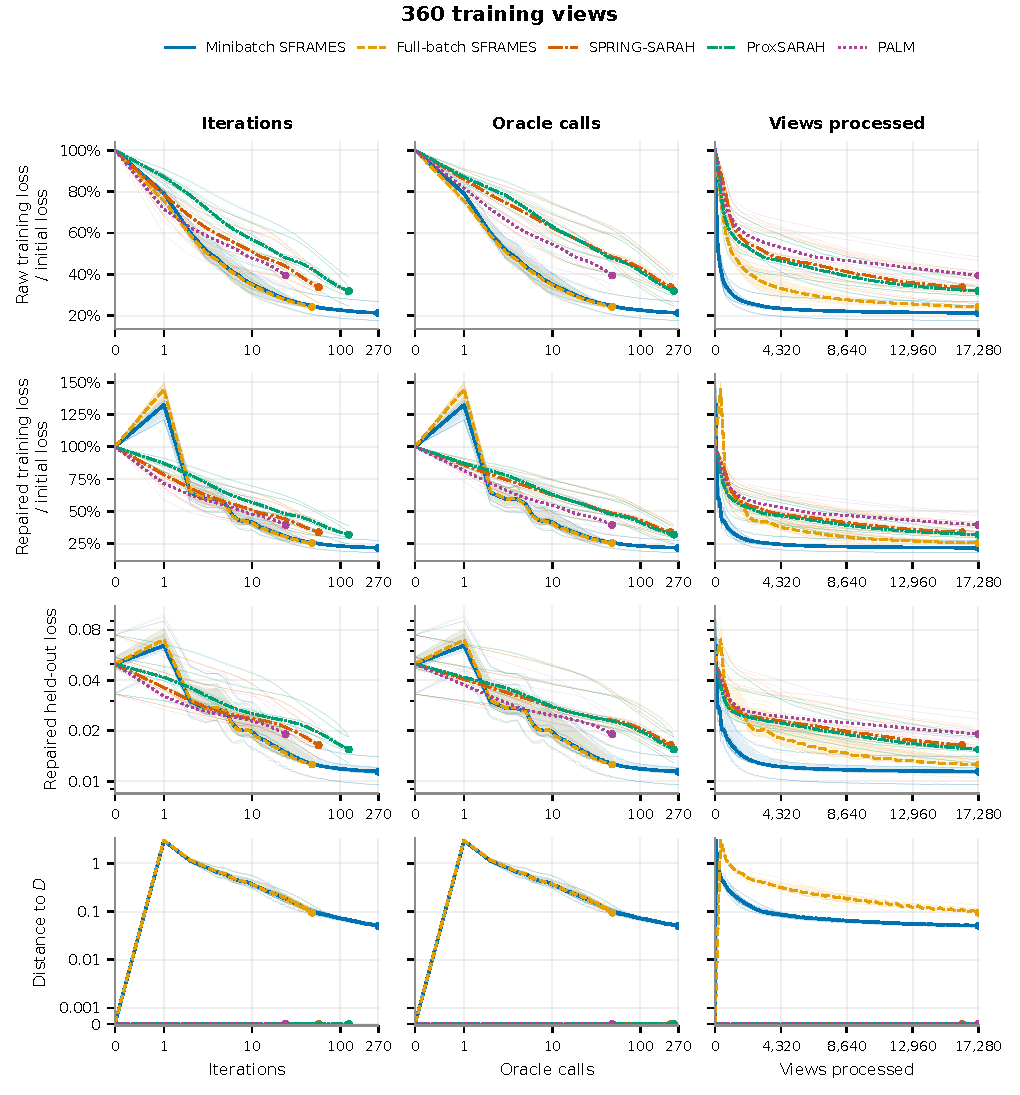
\includegraphics[width=\linewidth]{trajectories_360.pdf}
 \caption{Trajectories with \(360\) training views. Thin lines show
 individual runs, recorded at every update. Bold lines take median work
 and metric at the same iteration, first over seeds within slices and
 then across six slices. Bands show the middle \(50\%\) of slice medians
 for SFRAMES. Training losses are normalized by their initial values.}
 \label{fig:ct-trajectories-360}
\end{figure}

\begin{figure}[p]
 \centering
 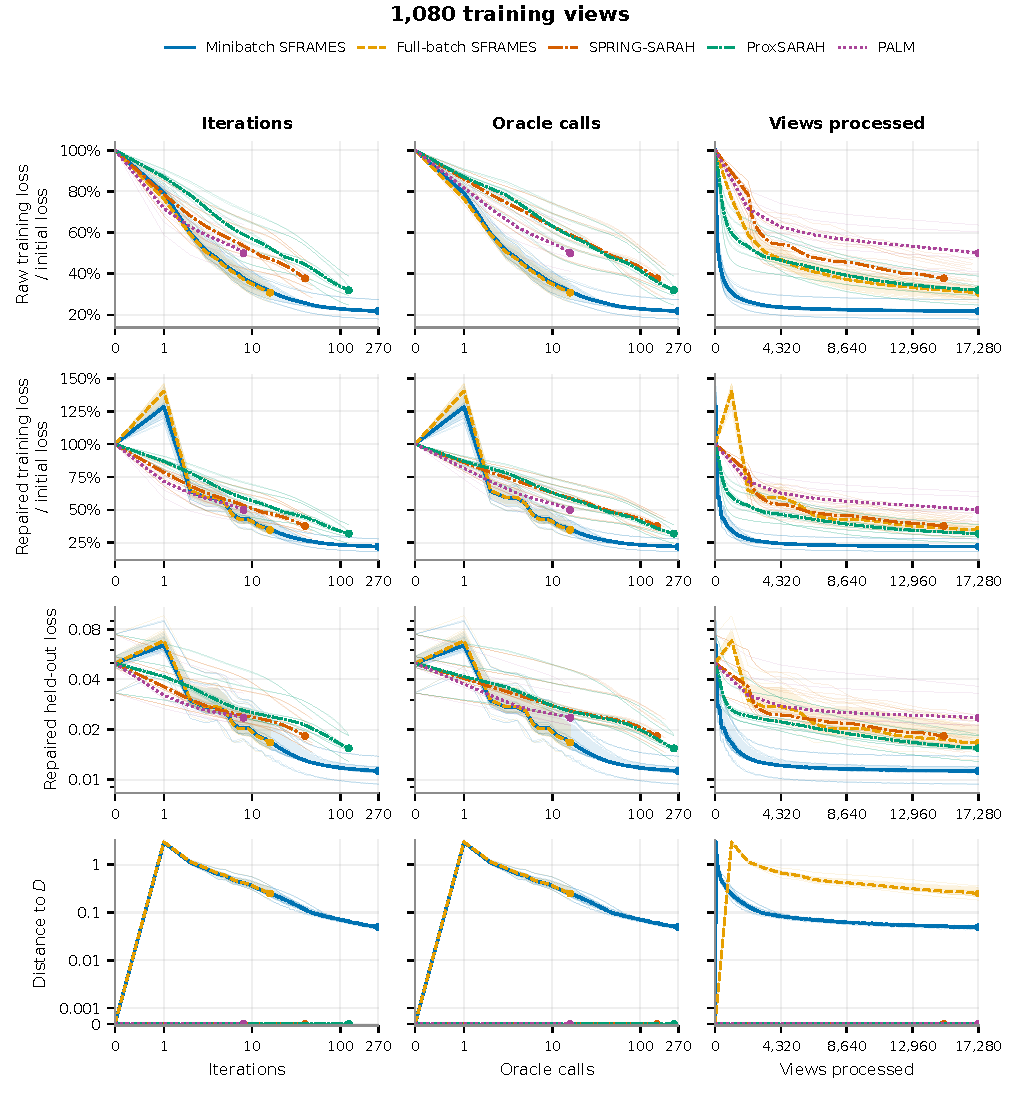
\includegraphics[width=\linewidth]{trajectories_1080.pdf}
 \caption{Trajectories with \(1{,}080\) training views, using the same
 metrics and summaries as Figure~\ref{fig:ct-trajectories-360}. The three
 projection baselines coincide at zero orthant distance.}
 \label{fig:ct-trajectories-1080}
\end{figure}

\clearpage
\subsection{Experimental protocol}
\label{subsec:ct-protocol}

We use measured fan-beam acquisitions from 2DeteCT \cite{detect}.
Mode~1 supplies the low-dose measurements, and the published Mode~2
reconstruction from a separate high-dose acquisition supplies the image
reference. Development uses slices \texttt{04300} and \texttt{03150}.
Evaluation uses \texttt{03041}, \texttt{03381}, and \texttt{03611} from
Mix~2, and \texttt{03791}, \texttt{04131}, and \texttt{04931} from Mix~3.
Each group contains cross sections of one specimen tube.

We discard the repeated final angle, sum adjacent detector cells, subtract
the similarly binned dark field, and divide by the mean flat field after
dark correction. Taking the negative logarithm with a transmission floor
of \(10^{-6}\), then reversing the detector axis, gives
\(3{,}600\times956\) sinograms in the DeepInverse convention
\cite{deepinv}. The floor is inactive for all selected acquisitions.
ASTRA~2.5.0 applies the FP32 CPU \texttt{line\_fanflat} projector
\cite{astra}, while the factor arithmetic is FP64. The source-to-origin
and origin-to-detector distances are \(431.019989\) and \(97.980499\)~mm,
with detector spacing \(0.1496\)~mm. The square field has width
\(116.528143\)~mm and center \((-0.113797,-0.113797)\)~mm, and view
\(i\) has angle \(\pi-2\pi i/3600\). We vertically flip the
\(1024\times1024\) reference, divide by its native voxel width
\(0.113797\)~mm, and average \(2\times2\) blocks.

For \(i\in\{0,\ldots,3599\}\), the training sets select
\(i\bmod10=0\) for \(N=360\) and
\(i\bmod10\in\{0,3,6\}\) for \(N=1{,}080\). Both reserve the
\(360\) views with \(i\bmod10=9\) for evaluation. Calibration uses the
\(120\) training views with \(i\bmod30=0\), shared across both sizes.
The stochastic methods use three paired oracle seed labels
\(202,203,204\), with generator seeds offset by \(100{,}000\).
Development uses label \(110\). PALM and full-batch SFRAMES run once
per slice and training size and serve as shared deterministic references.

All methods start from the same calibrated factors in \(C\cap D\).
Writing \(P_J\) for the calibration operator, we divide
\((P_J^\ast y_J)_+\) entrywise by \(P_J^\ast P_J\mathbf1\), with
denominator floor \(10^{-3}\) times its maximum. A nonnegative
SVD-based factorization gives rank-\(64\) factors, perturbed by
\(10^{-3}\) times each factor's RMS times uniform \([0,1)\) entries.
We fit a least-squares amplitude on the calibration views with lower bound
\(10^{-6}\), applying its square root to both factors. Calibration uses
seed \(110\) in development and \(201\) in evaluation. The numerical LMO retains singular values above
\(\varepsilon_{\rm mach}\max(\operatorname{shape}G)\sigma_{\max}(G)\).

SPRING--SARAH \cite{spring} alternates factor updates with steps
\(a/L_U,a/L_V\). Each block independently refreshes with probability
\(1/q\), starting from a full gradient, and otherwise uses a paired
\(64\)-view SARAH difference. ProxSARAH \cite{proxsarah} uses joint steps
\(a/(L_U+L_V)\), \(256\)-view snapshots followed by \(m\) recursive
\(64\)-view updates, and relaxation \(0.8\). Both terms of each recursive
difference use the same sampled views. PALM \cite{palm} uses full gradients
with alternating steps \(a/L_U,a/L_V\). Proximal steps project each factor
onto its spectral ball intersected with the nonnegative orthant. A feasible
single-set projection is accepted directly. Otherwise Dykstra iterations
use a primal--dual certificate, requested distance tolerance
\(10^{-8}(k+1)^{-1.1}\), at most \(2{,}000\) iterations, and checks at the
first, every fifth, and final iteration, with a floating-point allowance.

\begin{table}[!htbp]
\centering
\caption{Development hyperparameters. The two SFRAMES rows list complete Cartesian grids for the joint smoothing multiplier and step prefactor, with the selected pair in the final column. Baseline settings are retained from their original development searches.}
\label{tab:ct-settings}
\small
\setlength{\tabcolsep}{4pt}
\begin{tabular}{@{}lll@{}}
\toprule
Method and parameter & Values tested & Selected \\
\midrule
\shortstack[l]{Minibatch SFRAMES\\ $(c_\beta,\gamma_0)$} & \shortstack[l]{$c_\beta\in\{0.25, 1, 4, 16, 64\}$\\ $\gamma_0\in\{0.05, 0.1, 0.16, 0.25, 0.5, 0.8\}$} & $(16,0.1)$ \\
\shortstack[l]{Full-batch SFRAMES\\ $(c_\beta,\gamma_0)$} & \shortstack[l]{$c_\beta\in\{0.25, 1, 4, 16, 64\}$\\ $\gamma_0\in\{0.05, 0.1, 0.16, 0.25, 0.5, 0.8\}$} & $(16,0.1)$ \\
SPRING--SARAH, $(a,q)$ & (0.7,16), (1.1,16), (1.6,16), (1.1,8), (1.1,32) & (1.6,16) \\
ProxSARAH, $(a,m)$ & (0.9,12), (1.5,12), (2.3,12), (1.5,6), (1.5,24) & (2.3,12) \\
PALM, $a$ & 0.6, 1.1, 1.6, 2.3 & 2.3 \\
\bottomrule
\end{tabular}
\end{table}
We jointly select \((c_\beta,\gamma_0)\) for each SFRAMES variant by the
smallest median repaired-to-initial training-loss ratio over the two
development slices and both training-view counts at
\(8{,}640\) views per direction.
When a selected pair lies on a grid edge, that dimension is extended while
retaining the full Cartesian product. Table~\ref{tab:ct-settings} gives the
final tested grids, and Figure~\ref{fig:ct-joint-selection} shows their
observed scores. Held-out views and reference images do not enter selection.
The initial calibration fixed \(c_\beta=1\) by this curvature-scaling
heuristic and varied only \(\gamma_0\). All SFRAMES evaluation results
reported here use the joint selection.
The SPRING--SARAH, ProxSARAH and PALM step multipliers are at the upper
edges of their original grids.

Evaluation permits \(17{,}280\)
forward and adjoint views each. Counters include all gradient evaluations,
refreshes, snapshots and both terms of recursive differences. A gradient call
returns a joint or block gradient. Each iteration updates both factors.
Data processed is \(W=\sum_{\ell=1}^G|B_\ell|\), counting the views in
each of the \(G\) gradient calls. One processed view uses one forward and
one adjoint over all \(956\) bins. Diagnostic forward projections are
evaluated separately. Evaluation records the initialization and every
optimizer update, and tables use each run's last iterate within budget.
Paired percentage changes are computed within each seed pair, then summarized
by medians over seeds within slices and across slices.

\begin{figure}[!htbp]
 \centering
 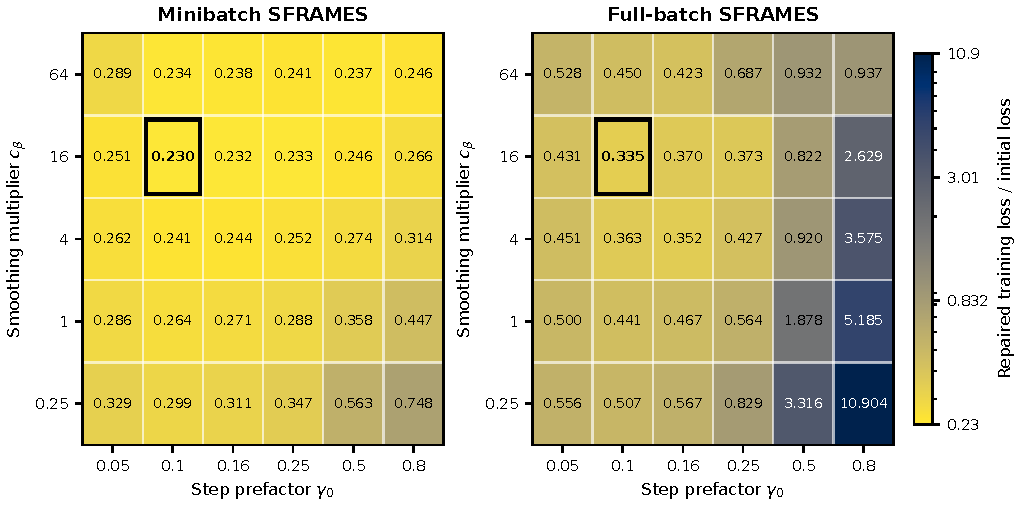
\includegraphics[width=\linewidth]{joint_selection.pdf}
 \caption{Joint development search. Each cell gives the median repaired
 training loss relative to initialization across the two development slices
 and both training-view counts. Here
 \(\beta_0=c_\beta/\max(L_U,L_V)\). Boxes mark the selected pairs, and lower
 values are better. The color scale is shared and logarithmic.}
 \label{fig:ct-joint-selection}
\end{figure}
